\newpage

\section{Przygotowanie próbek do badań}

\subsection{Przyrząd pomiarowy, rysunek, opis}
Schemat układu pomiarowego do badania widma ramnowskiego w funkcji polaryzacji światła padającego i promieniowania rozproszonego został przedstawiony na rysunku niżej:
\begin{figure}[H]
	\begin{center}
		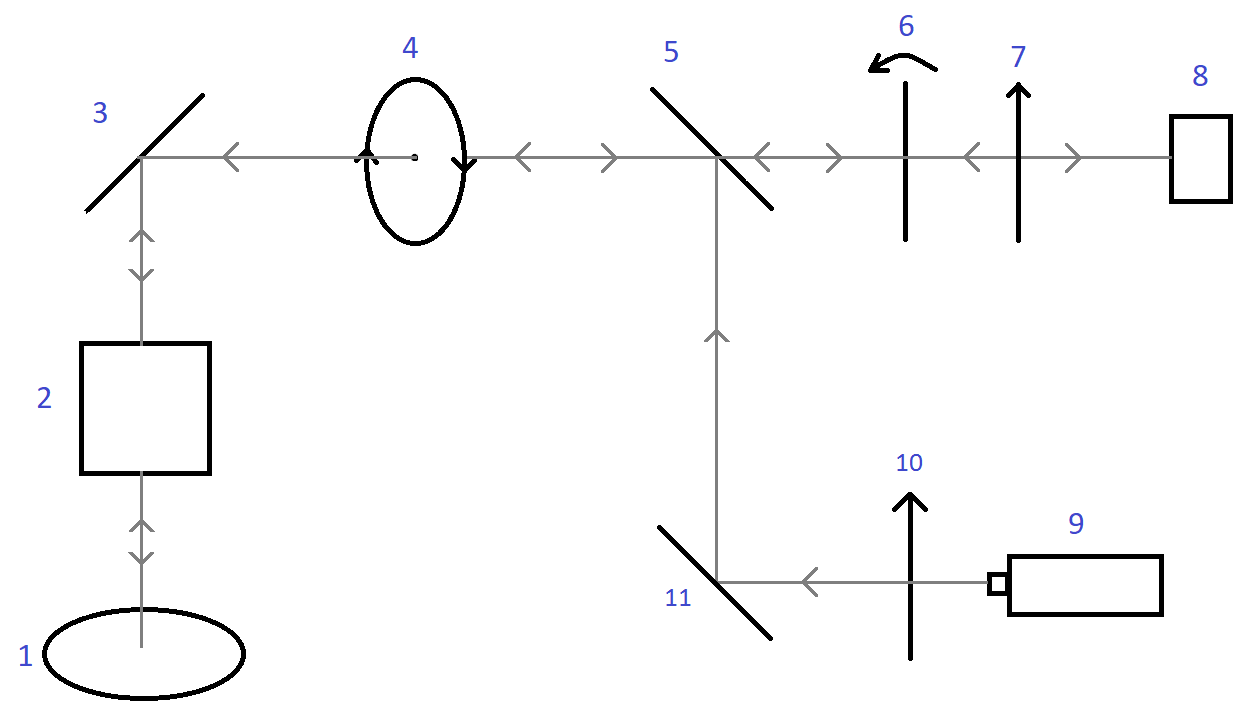
\includegraphics[width=1.0\linewidth]{Przygotowania/Uklad-pomiarowy.png}
		\caption{Schemat układu pomiarowego, wykorzystywanego w tej pracy.}
	\end{center}
\end{figure}
Główne elementy układu pomiarowego zostały zaznaczone cyframi arabskimi na rysunku wyżej i są to:
\begin{itemize}
	\item 1 - Badana próbka, $\alpha$-$\mathbf{Ga_{2}S_{3}}$;
	\item 2 - Mikroskop;
	\item 3, 11 - Lustra przekierowujące wiązkę światła;
	\item 4 - HWP\footnote{HWP z angielskiego ''Half-wave plate'' czyli  płytka półfalowa}, nazwa skrócona ''półfalówka'';
	\item 5 - Płytka pólprzepuszczająca;
	\item 6 - HWP 90$^{\circ}$, ustawiona tak że przekręca polaryzację o 90$^{\circ}$;
	\item 7, 10 - Polaryzatory;
	\item 8 - Detektor;
	\item 9 - Laser argonowy 514 nm;
	\item 12 - Monochromator, siatka dyfrakcyjna;
\end{itemize}

Jako promieniowanie pobudzające użyto długości fali 514 nm, emitowanej przez laser argonowy (9), wiązka pobudzająca laserowa przechodzi przez pionowo ustawiony polaryzator (10). Chociaż fala elektromagnetyczna emitowana laserem jest już spolaryzowana, polaryzator (10) zapewnia większy stopień jej polaryzacji. Dalej fala elektromagnetyczna odbija się od zwierciadła (11) i trafia na płytkę półprzepuszczającą (5). Następnie odbija się od tej płytki i przechodzi przez HWP (4). Jeśli oś ''półfalówki'' jest obrócona o kąt $\alpha$ wtedy po przejściu przez ''półfalówkę'' polaryzacja fali elektromagnetycznej zostaje przekręcona o kąt 2$\alpha$. Dalej fala przechodzi przez mikroskop (2) i trafia na próbkę (1). W wyniku oddziaływania z drganiami fali elektromagnetycznej z fononami powstaje fala rozproszona ramanowsko. Część tej fali trafia na zwierciadło (3), odbija się od tego zwierciadła i przechodzi przez ''półfalówkę'' (4). Teraz ''półfalówka'' względem światła rozproszonego ma oś skręconą o kąt $-\alpha$. Po przejściu przez (4) polaryzacja rozproszonej fali elektromagnetycznej zostaje obrócona o -2$\alpha$. Dalej światło rozproszone ramanowsko trafia do ''półfalówkę'', gdzie oś ''półfalówki'' jest przekręcona na stałe o kąt 45$^\circ$ wobec tego po przejściu przez (6)promieniowanie rozproszone ma polaryzację obróconą o kąt 90$^\circ$. Po przejściu przez polaryzator (7) zostaje wybrana tylko określona polaryzacja fali rozproszonej. Następnie fala elektromagnetyczna rozproszona trafia na układ monochromatora i dalej na detektor z kamerą CCD. Polaryzator (7) jest po to aby wybrać światło rozproszone tylko o określonej polaryzacji.

Pomiar odbywał się w dwóch konfiguracjach:
\begin{itemize}
	\item VV - rejestrowane promieniowanie rozproszone miało polaryzację w takim samym kierunku jak światło pobudzające\footnote{Światło emitowane laserem}. Pomiar wtedy odbywał się bez HWP 90$^{\circ}$ (6).
	\item VH - rejestrowane promieniowanie rozproszone było spolaryzowane w kierunku prostopadłym do światła pobudzającego. Pomiar wtedy odbywał się z HWP 90$^{\circ}$
\end{itemize} 

Główne parametry pomiaru:
\begin{itemize}
	\item Czas pomiaru 30 sek;
	\item Środek detektora 1040 $cm^{-1}$;
	\item Moc lasera 10 \% z $\frac{3}{4}$ mocy maksymalnej;
	\item Polaryzacja lasera normalna;
	\item Długość fali 514 nm;
	\item Kąt polaryzacji w kolejnym kroku pomiarowym zmieniano o 5$^{\circ}$;
	\item Konfiguracja VV bez elementu (6) rys. 22. Konfiguracja VH z elementem (6).
	\item Oprogramowanie \textit{Wire} 4.2.
\end{itemize}

\begin{figure}[H]
	\begin{center}
		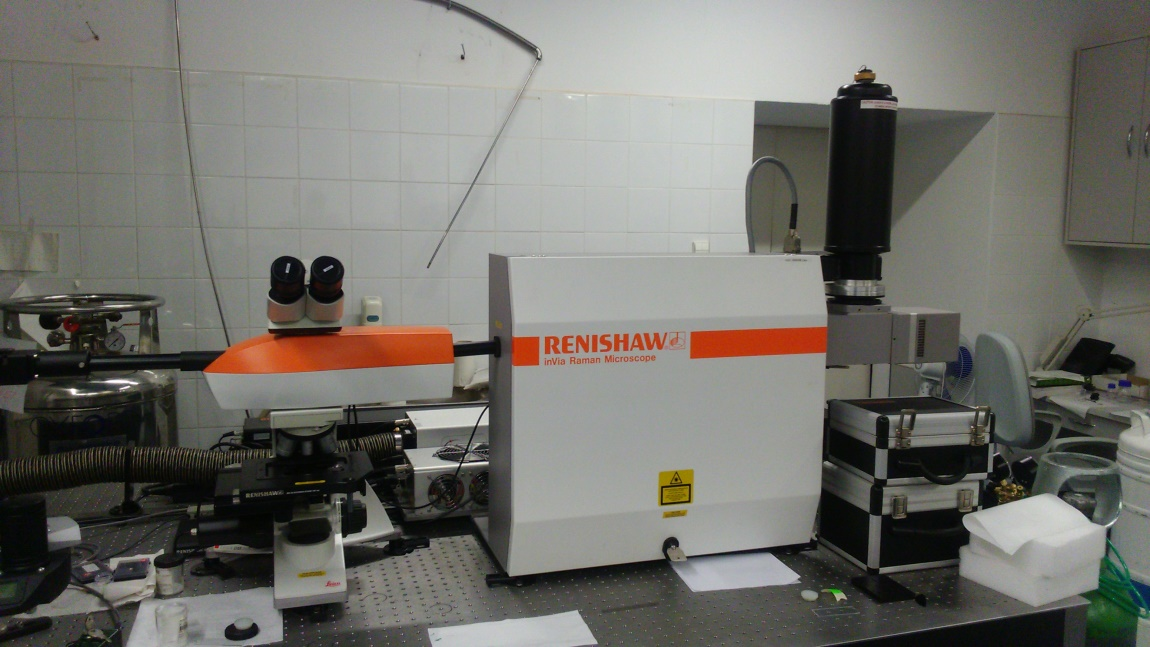
\includegraphics[width=0.8\linewidth]{Przygotowania/Spektroskop.png}
		\caption{Zdjęcie układu pomiarowego na którym wykonywane były pomiary ramanowskie.}
	\end{center}
\end{figure}

Płytka podłożowa $\mathbf{GaP}$ miała wymiary 3mm x 2mm x 1mm. Kryształki $\mathbf{Ga_{2}S_{3}}$, które zostały wytworzone na tej płytce były rzędu kilku mikrometrów. Próbka do badań polaryzacyjnych powinna być monokryształem, dla tego do badań wyselekcjonowano kryształki w kształcie sześciokątów o płaskiej powierzchni ustawionej prostopadle do padającej wiązki laserowej.

Pierwsze pomiary ramanowskie zostały wykonane na takich kryształkach, jednak obecność pików podłoża $\mathbf{GaP}$ w pewny stopniu utrudniała analizę otrzymanych wyników. W kolejnym etapie kryształki $\mathbf{Ga_{2}S_{3}}$ zostały $"$zdrapane$"$ i przeniesione na szklaną płytkę.

Pomiary polaryzacyjne były wykonywane w jednej wielogodzinnej sesji pomiarowej. Uniknięto w ten sposób błędów związanych z rozkalibrowaniem układu pomiarowego, a także ze zmianę orientacji próbki pomiarowej, względem wiązki laserowej.

Pomiary były wykonane za pomocą spektrometru RENISZAW InVia. Pomiary były wykonywane w warunkach normalnych.

\subsection{Technologia wytwarzania warstwy $\mathbf{Ga_{2}S_{3}}$} 

$\mathbf{Ga_{2}S_{3}}$ posiada odmienną strukturę krystaliczną od $\mathbf{GaS}$ – żadna faza krystaliczna siarczku galu(III) nie wykazuje budowy warstwowej. W związku z tym otrzymywanie cienkich warstw $\mathbf{Ga_{2}S_{3}}$ nie jest możliwe w procesie eksfoliacji i wymaga zastosowania innych metod (np. CVD, MBE).

Warstwy $\mathbf{Ga_{2}S_{3}}$ były otrzymywane poprzez reakcję par siarki z płytkami krystalicznego fosforku galu. W ampule kwarcowej umieszczono krystaliczną płytkę $\mathbf{GaP}$\footnote{Płytka jest mała o wymiarach 5 x 3 x 1 mm.} oraz 1 mg krystalicznej siarki. Ampułę następnie zamknięto pod próżnią (<1 mbar) i wstawiono do pieca rurowego w taki sposób by płytka $\mathbf{GaP}$ była w środku strefy grzejnej. Następnie rozpoczęto ogrzewanie ampuły przy szybkości wzrostu temperatury $1^{\circ}/min$ aż do osiągnięcia temperatury 600$C^{\circ}$ Reakcję prowadzono przez 4 dni, po których piec wyłączono i pozostawiono do naturalnego wystygnięcia.

Próbki były wytwarzane w ramach współpracy z Wydziałem Chemicznym Politechniki Warszawskiej w laboratorium Związków Beztlenowych. Na rysunku poniżej przedstawione zostały zdjęcia z mikroskopu optycznego kryształków $\mathbf{Ga_2S_3}$ na których były wykonywane pomiary ramanowskie. Rysunek 23 a) przedstawia próbkę na podłożu $\mathbf{GaP}$, rysunej b)na podłożu szklanym. Rozmiar próbek użytych do badań był rzędu 5-10 mikrometrów. Strukturę warstwy $\mathbf{Ga_{2}S_{3}}$ na podłożu $\mathbf{GaP}$ w większej rozdzielczości uzyskano za pomocą SEM, przykładowe zdjęcia znajdują się na rysunku 24.

\begin{figure}[H]
	\begin{minipage}[h]{0.5\linewidth}
		\center{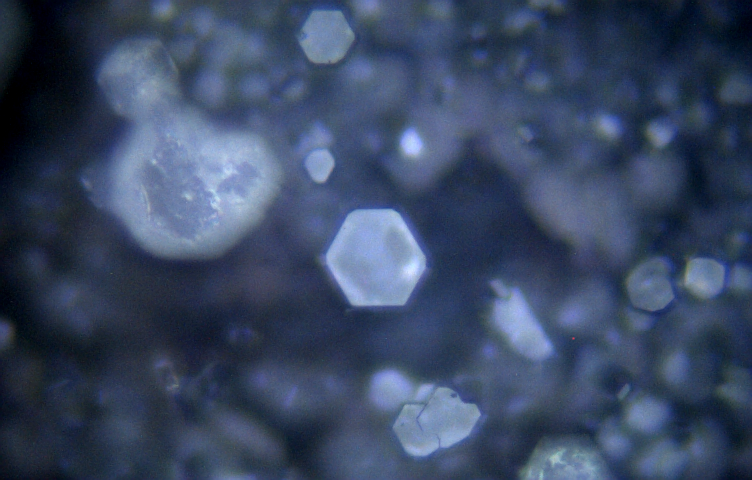
\includegraphics[width=0.8\linewidth]{Przygotowania/SLA39-50x-plytkiGa2S3.png}} \\ a) 
	\end{minipage}
	\hfill
	\begin{minipage}[h]{0.5\linewidth}
		\center{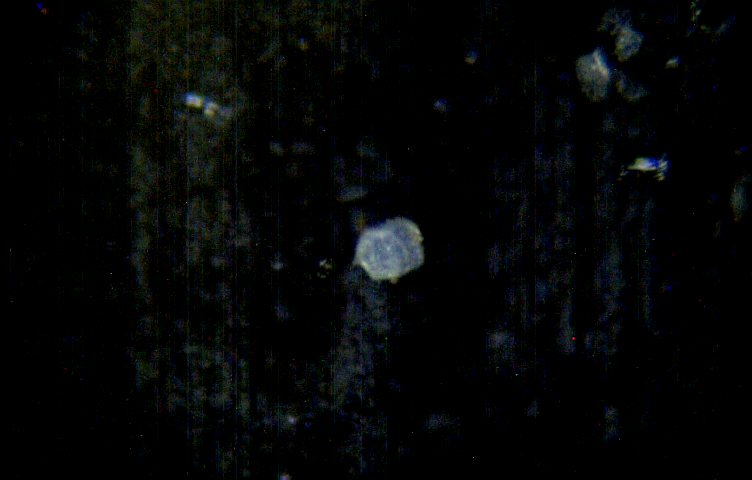
\includegraphics[width=0.8\linewidth]{Przygotowania/long50x.png}} \\b)
	\end{minipage}
	\caption{Zdjęcie z mikroskopu optycznego kryształku $\mathbf{Ga_{2}S_{3}}$ na podłożu $\mathbf{GaP}$ - a) oraz podłożu szklanym - b)}
\end{figure}

\begin{figure}[H]
	\begin{minipage}[h]{0.47\linewidth}
		\center{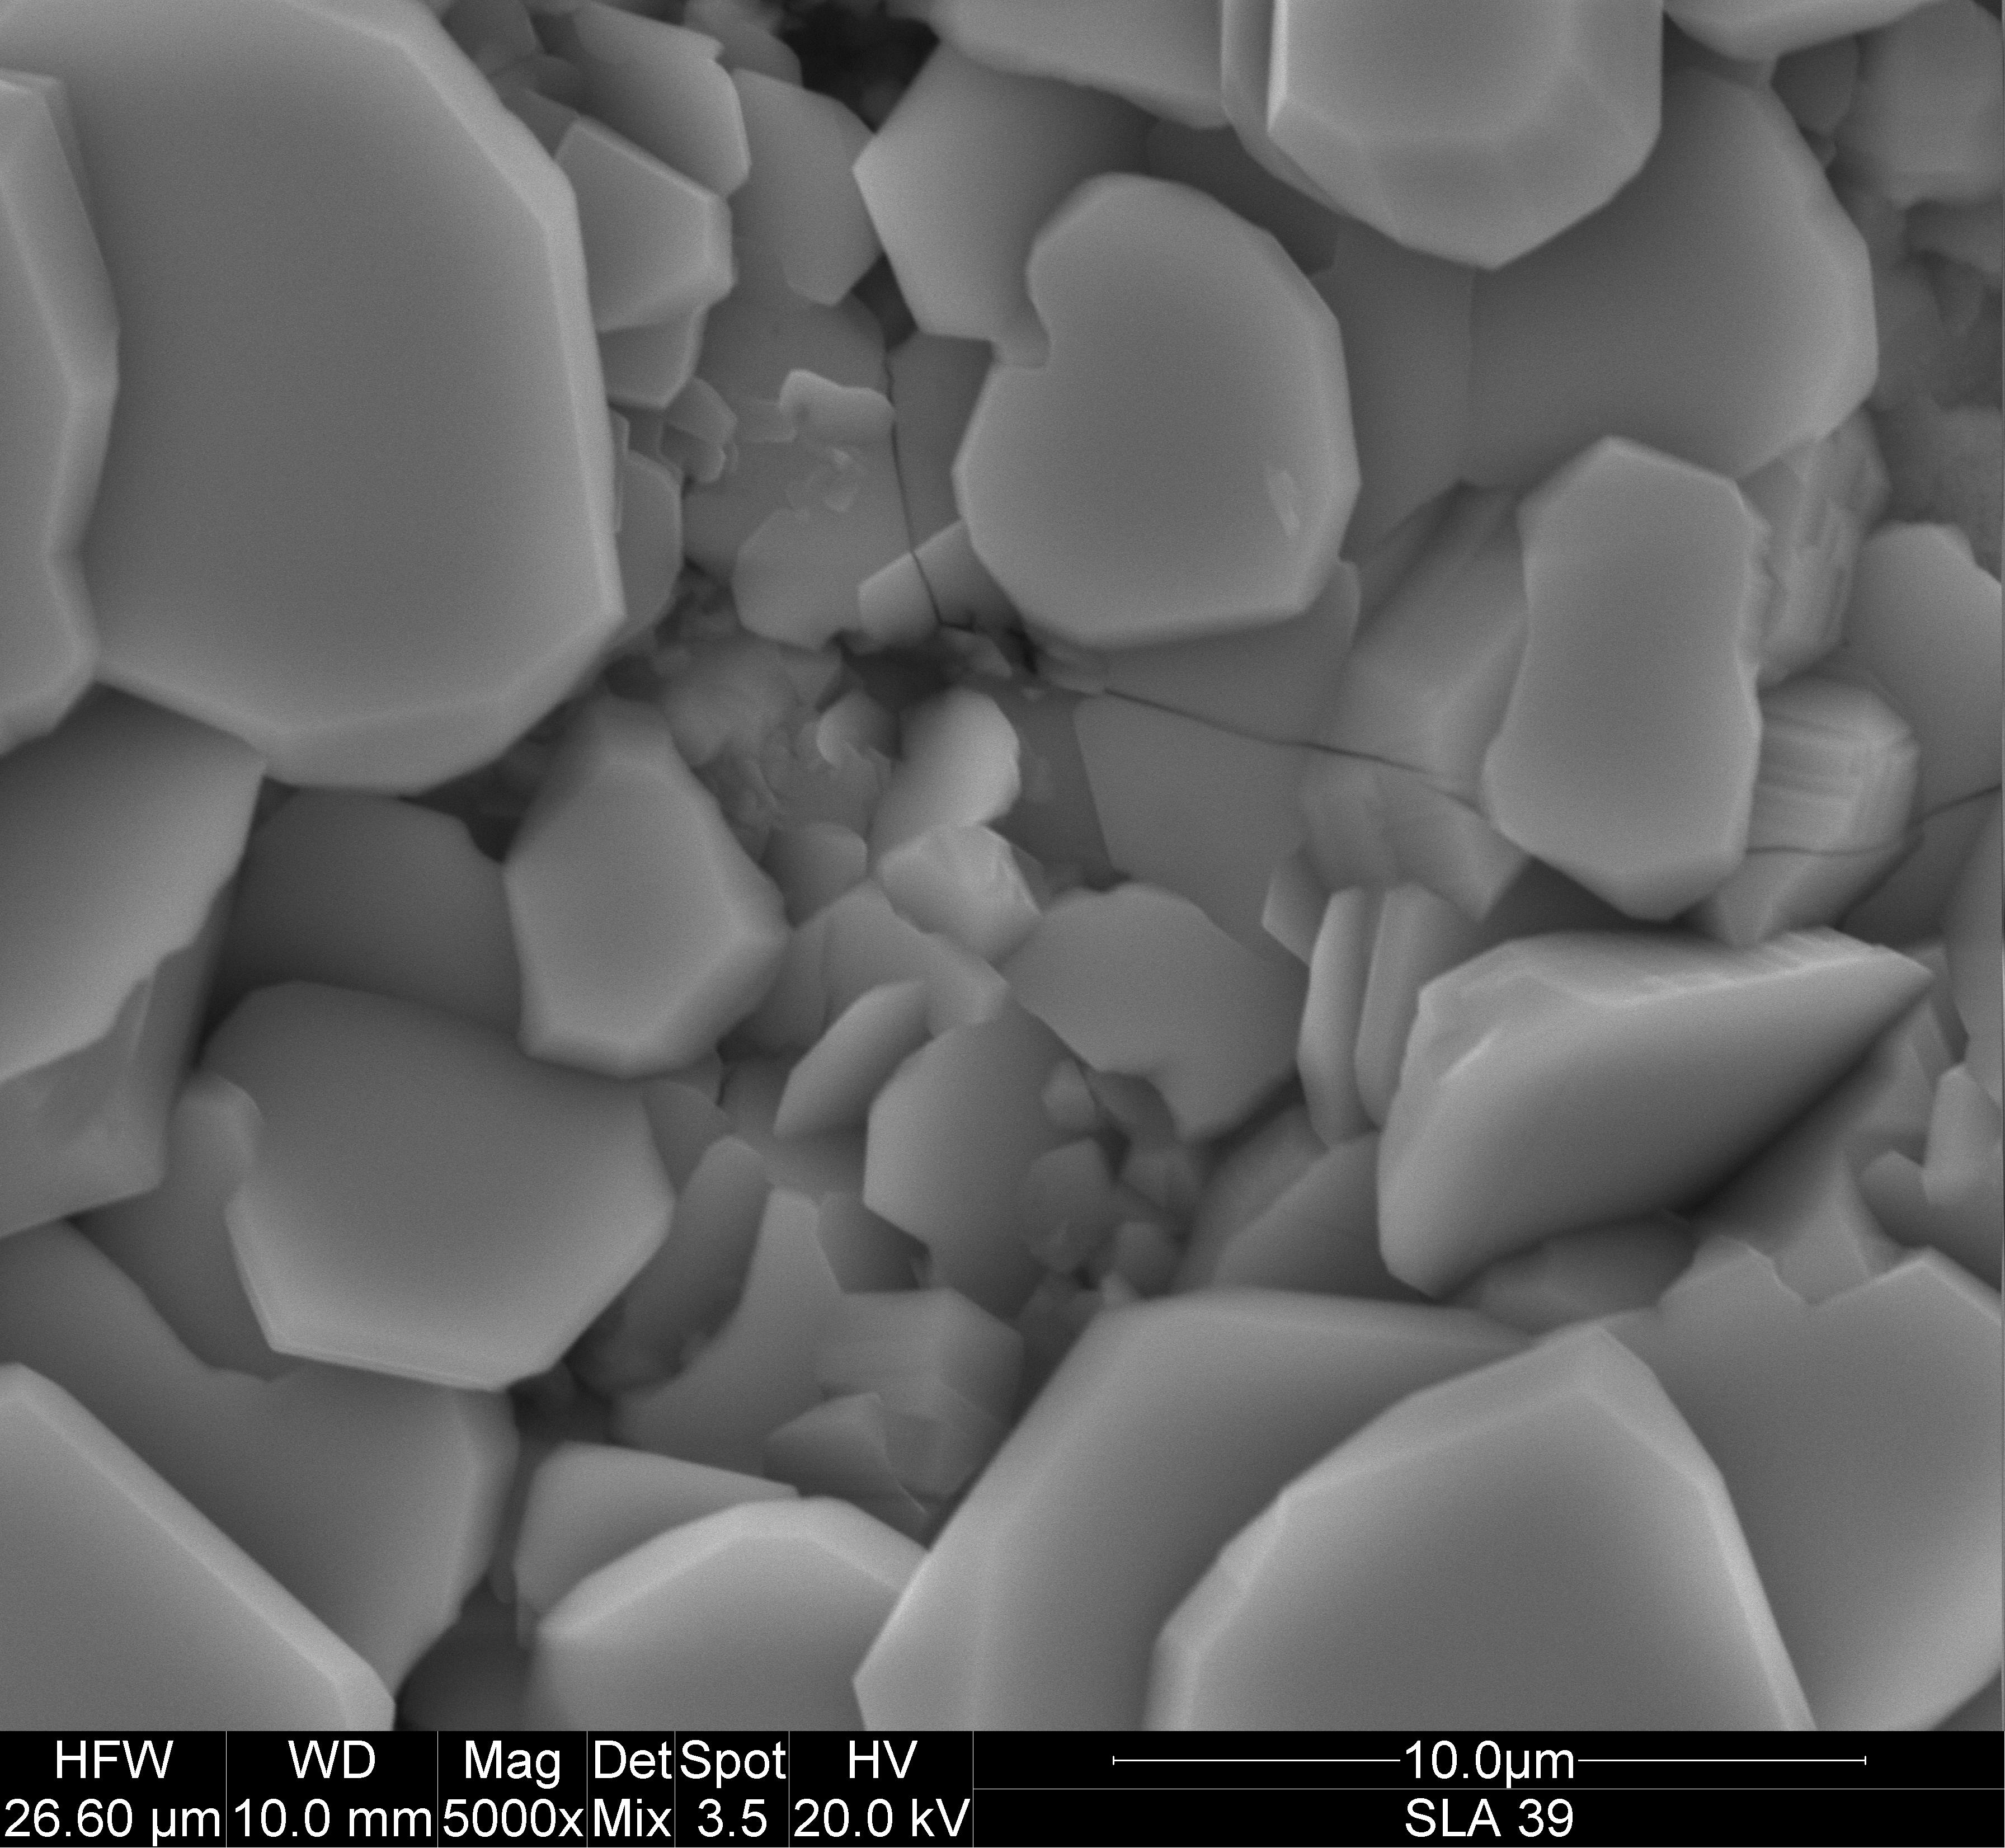
\includegraphics[width=0.7\linewidth]{Wlasciwosci/SLA39_MIX_5000.jpg}} \\a) 
	\end{minipage}
	\hfill
	\begin{minipage}[h]{0.47\linewidth}
		\center{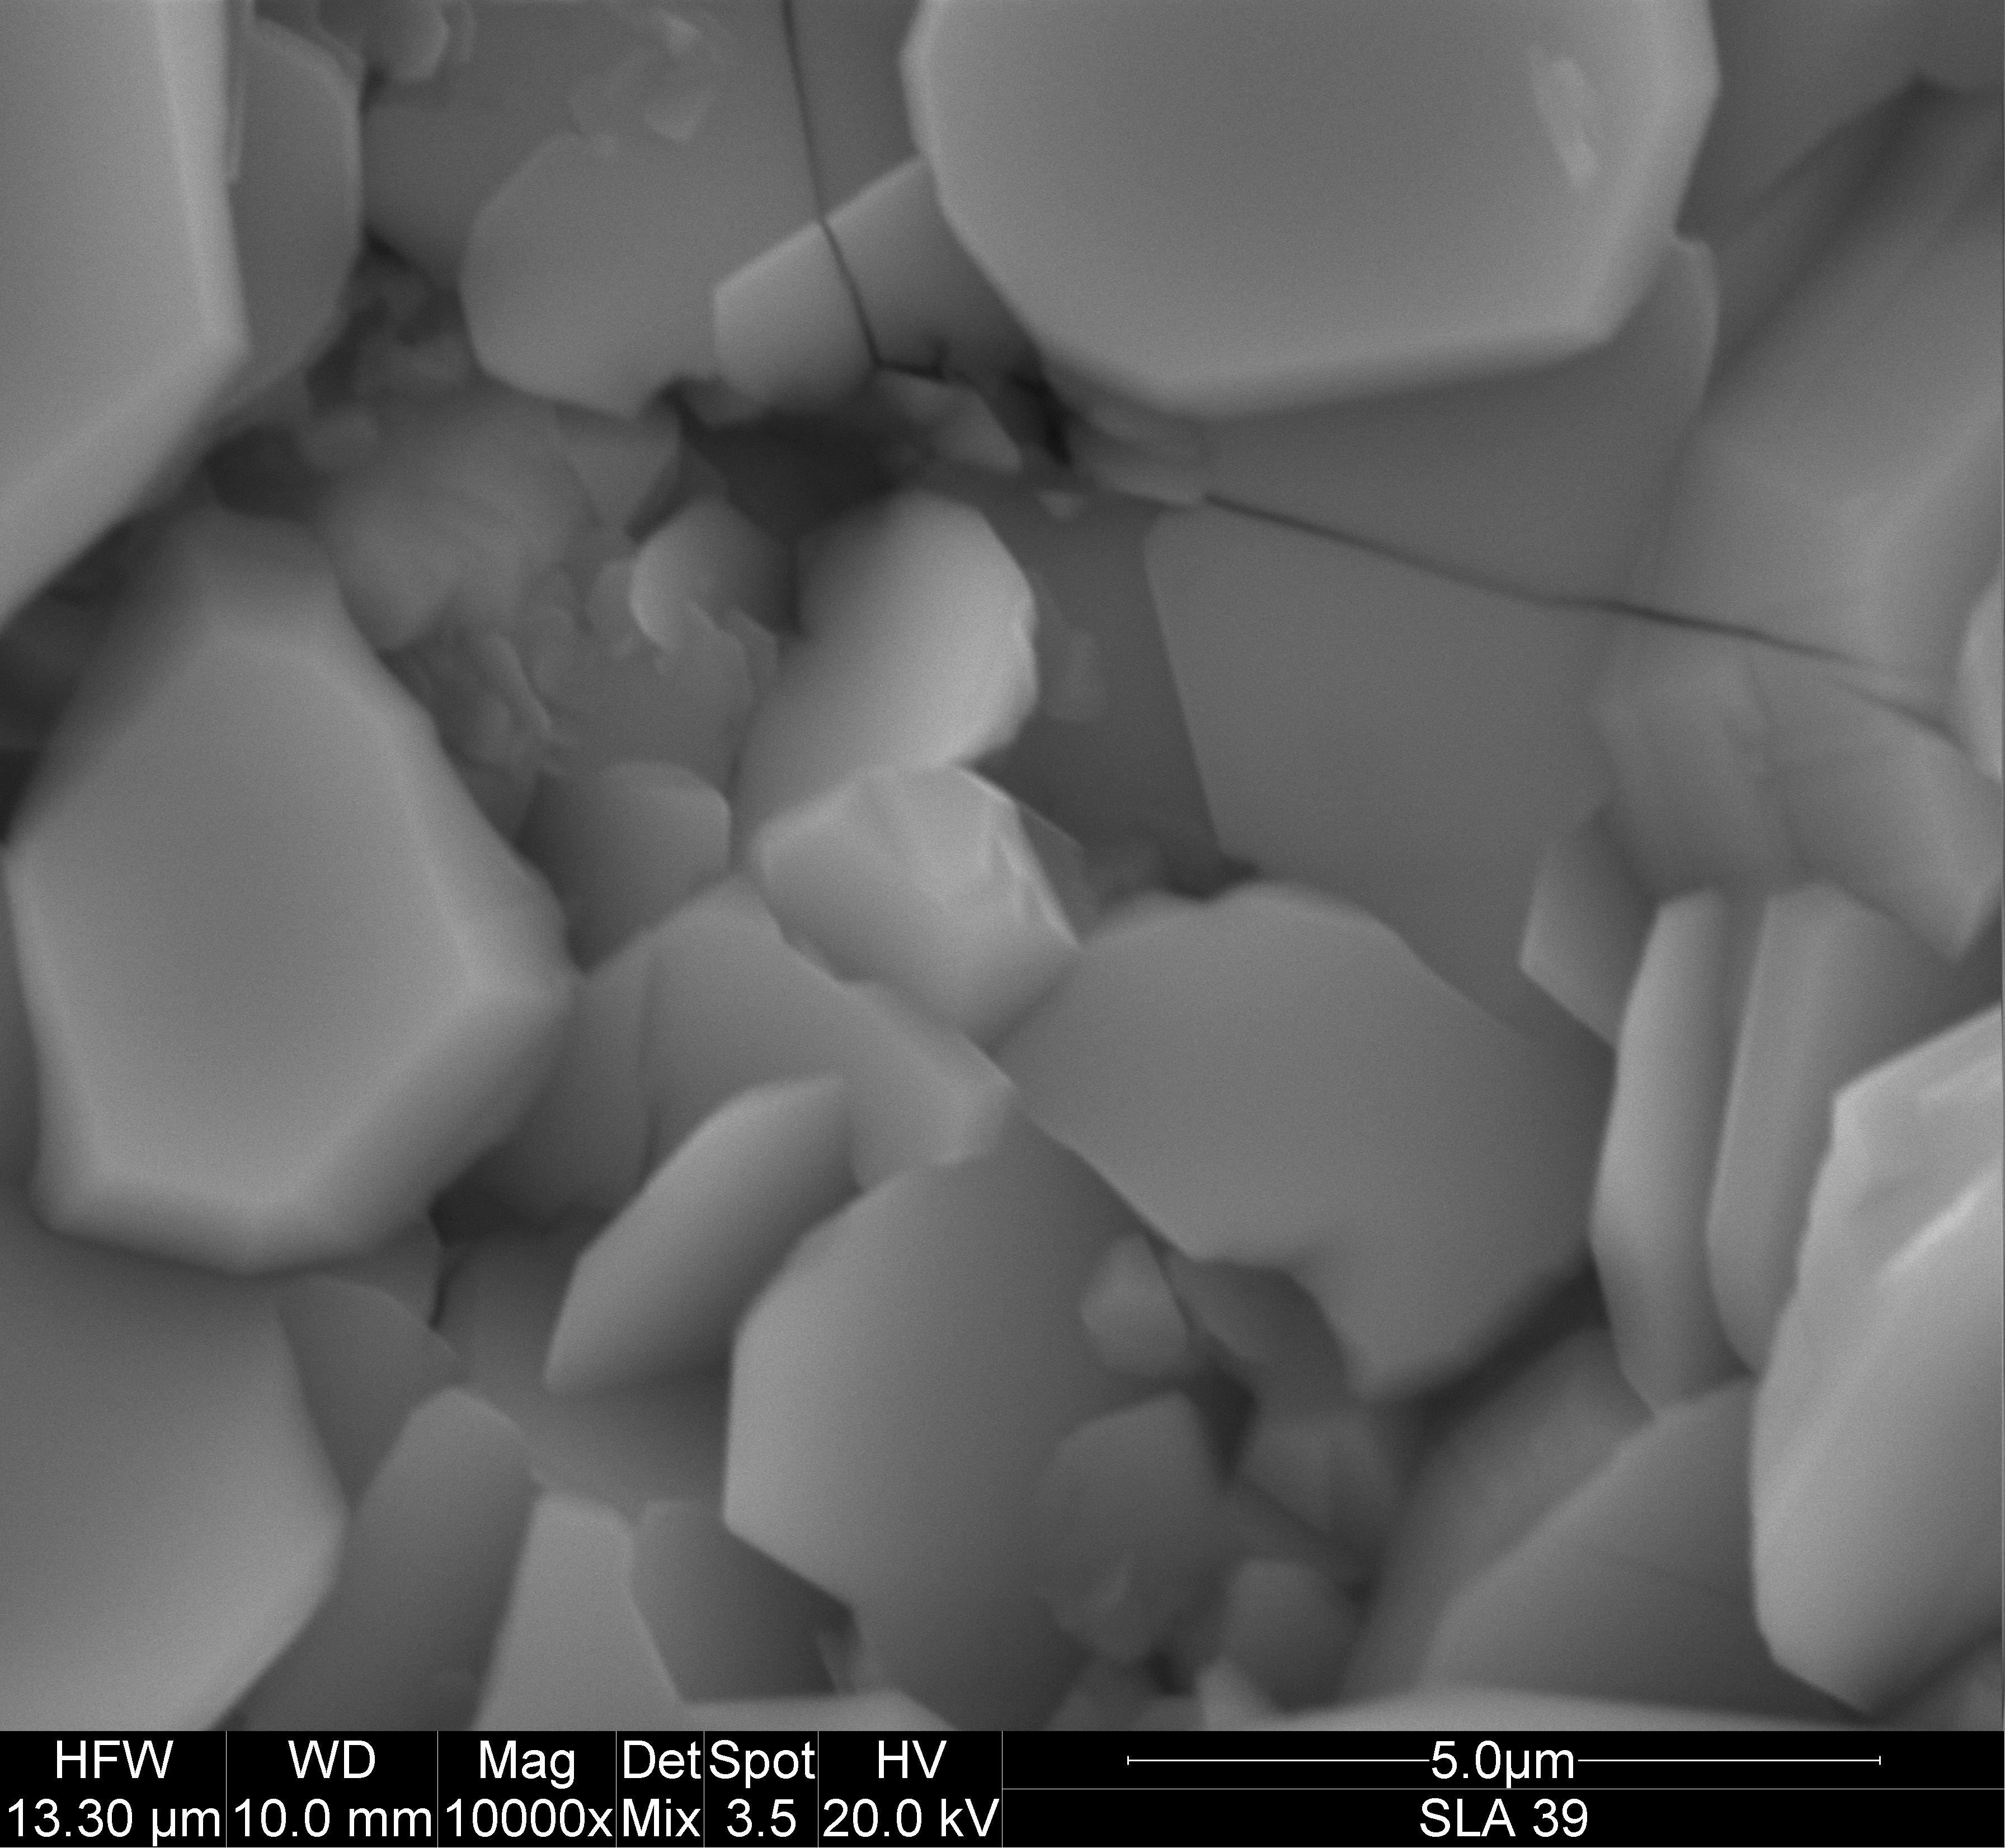
\includegraphics[width=0.7\linewidth]{Wlasciwosci/SLA39_MIX_10000.jpg}} \\b)
	\end{minipage}
	\caption{Na rysunku przedstawiono zdjęcia warstwy $\mathbf{Ga_{2}S_{3}}$ wykonanej za pomocą SEM przy powiększeniu : a) 5000 razy, b) 10000 razy [1].}
\end{figure}

\begin{figure}[H]
	\begin{center}
		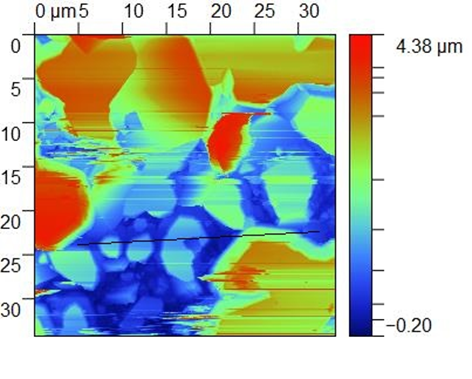
\includegraphics[width=0.55\linewidth]{Przygotowania/SEM.png}
		\caption{Skan z mikroskopu sił atomowych AFM przykładowej powierzchni $\mathbf{Ga_2S_3}$ na podłożu $\mathbf{GaP}$ [36].}
	\end{center}
\end{figure}

Topografię wytworzonej warstwy Ga2S3 na podłożu GaP badano również za pomocą mikroskopu sił atomowych. Przykładowe zdjęcie z AFM przedstawiono na rysunku 25. Analiza profili grubości pokazała, że warstwy te miały grubość w zakresie około od kilkuset nanometrów do około dwóch mikrometrów.
























 